\documentclass[12pt, a4paper]{report}
\usepackage{minted}
\usepackage[utf8]{inputenc}
\usepackage[T1]{fontenc}
\usepackage[polish]{babel}
\usepackage{titling}
\usepackage{graphicx}
\usepackage{lmodern}
\usepackage[a4paper, margin=1in, top=0.5in, bottom=1in]{geometry}
\usepackage{footnote}
\usepackage{float}
\usepackage{listings}
\usepackage{xcolor}
\usepackage{amsmath}
\usepackage{geometry}
\usepackage{longtable}
\usepackage{booktabs}
\usepackage[colorlinks=true, linkcolor=black, urlcolor=purple]{hyperref}

\lstdefinelanguage{json}{
    basicstyle=\ttfamily\small,
    keywordstyle=\color{blue},
    stringstyle=\color{green!50!black},
    commentstyle=\color{gray},
    stepnumber=1,
    numbersep=5pt,
    showstringspaces=false,
    breaklines=true,
    frame=single,
    morestring=[b]",
    morecomment=[l]{//},
    moredelim=[s][\color{blue}]{:}{,},
    backgroundcolor=\color{lightgray}
}

\lstset{
    basicstyle=\ttfamily\small,
    keywordstyle=\color{blue},
    commentstyle=\color{gray},
    frame=single,
    breaklines=true
}

\setlength{\parindent}{1cm}
\setlength{\parskip}{0cm}

% notes:
% - In polish we write titles of projects, chapters, sections with only first letter of first word large

\title{
``Sprawozdanie z projektu BigData\\ 
Predykcja cen samochodów używanych''
}
\author{
    Mateusz Grzybek 240678\\
    Kamil Młynarczyk  240757
}
\date{\today}

\begin{document}

%Title page definition
\begin{titlepage}
    \centering

    % University information
    {\Huge Politechnika Łódzka \\[0.5cm]}
    {\Large Wydział Elektrotechniki Elektroniki Informatyki i Automatyki \\[0cm]}
    
\includegraphics[width=0.5\textwidth]{images/university_logo}
    {\\[0cm] sem, zimowy, r ak. 2024/2025 \\[1cm]}
    
    % Project information
    {\Large \textbf{
        Sprawozdanie z projektu BigData\\ 
        „Predykcja cen samochodów używanych” \\[0.2cm]
    }}
    
\includegraphics[width=0.3\textwidth]{images/project_logo.png}
    {\\[0.3cm]}
    % Author information
    {\Large Mateusz Grzybek 240678 \\[0.2cm] Kamil Młynarczyk 240757 \\[1cm]}

    % Publication date
    {\Large \today}
\end{titlepage}

% Table of contents
\tableofcontents
\thispagestyle{empty}
\newpage

% chapter 1 - Introduction
\chapter{Wstęp}
\section{Założenia projektowe}
Celem projektu jest zaimplementowanie aplikacji webowej pozwalającej użytkownikom na predykcję 
ceny używanego samochodu na podstawie dostarczonego przez niego zestawu cech. Tematyka projektu
daje możliwość wykorzystania różnorodnych technologii z dziedziny uczenia maszynowego, rozwoju
aplikacji webowych, komunikacji pomiędzy serwisami, architektury oprogramowania oraz gromadzenia i 
przetwarzania danych. W celu zrealizowania przewidywanych funkcjonalności, aplikacja została
podzielona na cztery komponenty, każdy z nich odpowiedzialny za realizację innego aspektu
aplikacji.
\section{Komponenty}
\begin{itemize}
    \item Aplikacja kliencka --- Interfejs graficzny użytkownika.
    \item Pośrednik --- Komponent pośredniczący w komunikacji pomiędzy aplikacją kliencką i serwisem predykcyjnym
    \item Komponent komunikacyjny --- Komponent zawierający szyny danych, które są wykorzystywane do dostarczania i odbierania informacji od serwisu predykcyjnego
    \item Serwis predykcyjny --- Komponent dokonujący predykcji na podstawie dostarczonych danych, z wykorzytaniem nauczonego modelu.
\end{itemize}

\section{Konteneryzacja}
Wszystkie komponenty zostały skonteneryzowane za pomocą narzędzi
\textbf{Docker}\footnote{Narzędzie do tworzenia, uruchamiania i zarządzania aplikacjami w izolowanych środowiskach zwanych kontenerami.}
i \textbf{Docker Compose}\footnote{Narzędzie usprawniające zarządzanie wieloma kontenerami jednocześnie.}, co pozwala na uruchomienie projektu
bez konieczności dodatkowej konfiguracji.\ \textbf{Obrazy}\footnote{Gotowy do uruchomienia szablon do tworzenia kontenerów, zawierający system plików, aplikację i jej zależności.}
\textbf{kontenerów}\footnote{Lekkie, izolowane środowisko uruchomieniowe, które zawiera aplikację wraz z jej zależnościami.}
dla aplikacji klienckiej oraz pośrednika zostały zdefiniowane za pomocą
plików \textbf{Dockerfile}\footnote{Plik tekstowy zawierający zestaw instrukcji do zbudowania obrazu Docker.},
natomiast dla komponentu komunikacyjnego wykorzystano gotowe obrazy Apache Kafka i Zookeeper z rejestru Docker.io.
\section{Sposób uruchamiania}
\begin{enumerate}
\item Zainstalować Docker i Docker Compose.
\item Aplikacja kliencka --- Otworzyć katalog \texttt{frontend} i wewnątrz niego uruchomić skrypt \texttt{run.sh} lub uruchomić ręcznie komendy w terminalu. Wyłączenia kontenera można dokonać skryptem \texttt{clean.sh}.
\begin{itemize}
\item Skrypt \texttt{run.sh}:
\begin{lstlisting}[language=bash]
#!/bin/bash

# Builds docker image from local Dockerfile
# and sets image name to "frontend-image"
docker build -t frontend-image .

# Creates and runs container with name "frontend" from frontend-image
# in detached mode and container-host port mapping to 9091
docker run --name frontend -d -p 9091:9091 frontend-image
\end{lstlisting}

\item Skrypt \texttt{clean.sh}:
\begin{lstlisting}[language=bash]
#!/bin/bash

# Stops and removes the "frontend" container
docker stop frontend
docker rm frontend
\end{lstlisting}

\end{itemize}
\item Pozostałe komponenty --- Otworzyć katalog projektu i uruchomić komendę docker compose up.
Do wyłączenia kontenerów należy użyć komendy docker compose down.
\begin{lstlisting}
# Run containers
docker compose up

# Stop containers
docker compose down
\end{lstlisting}
    
\end{enumerate}
\newpage
\section{Dane}
Do utworzenia modelu predykcyjnego wykorzystany został zestaw danych
 \href{https://www.kaggle.com/datasets/taeefnajib/used-car-price-prediction-dataset}{``Used Car Price Prediction Dataset''}\footnote{https://www.kaggle.com/datasets/taeefnajib/used-car-price-prediction-dataset}
  z platfromy Kaggle. \\[1cm]
\textbf{Cechy zbioru danych:}
\begin{itemize}
    \item \textbf{brand} --- Marka lub nazwa firmy produkującej samochody.
    \item \textbf{mode} --- Model pojazdu.
    \item \textbf{model\_year} --- Rok produkcji pojazdu.
    \item \textbf{milage} --- Przebieg samochodu w milach.
    \item \textbf{fuel\_type} --- Rodzaj paliwa wykorzystywanego przez samochód.
    \item \textbf{engine} --- Typ silnika.
    \item \textbf{transmission} --- Typ skrzyni biegów.
    \item \textbf{ext\_col} --- Kolor zewnętrzny pojazdu.
    \item \textbf{int\_col} --- Kolor wnętrza pojazdu.
    \item \textbf{accident} --- Historia wypadków
    \item \textbf{clean\_title} --- Czy pojazd posiada czysty tytuł własności.
    \item \textbf{price} --- Cena samochodu według sprzedającego.
\end{itemize}

% chapter 2 - diagrams
\chapter{Diagramy}
\section{Diagram przypadków użycia}
\begin{figure}[H]
    \centering
    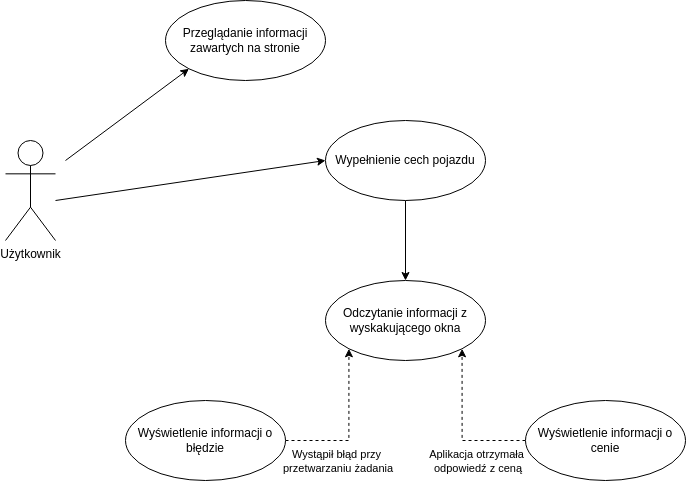
\includegraphics[width=1\textwidth]{diagrams/use_case_diagram.png}
    \caption{Przebieg interakcji użytkownika z aplikacją}
\end{figure}
\section{Diagram sekwencji zdarzeń}
\begin{figure}[H]
    \centering
    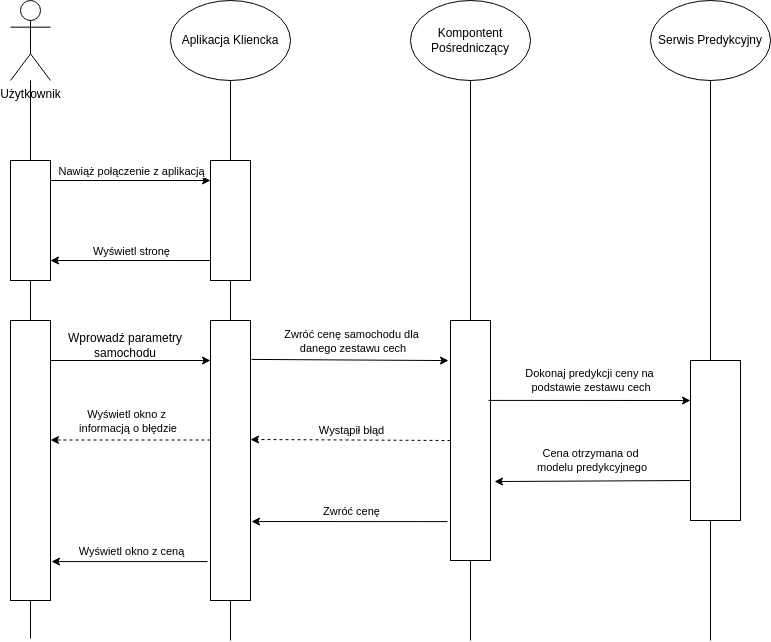
\includegraphics[width=1\textwidth]{diagrams/sequence_of_events_diagram.png}
    \caption{Przebieg operacji komponentów i działań użytkownika podczas procesu predykcji ceny samochodu}
\end{figure}


% chapter 3 - frontend
\chapter{Aplikacja kliencka}
\section{Opis}
Aplikacja kliencka stanowi pojedynczą stronę dostępną za pośrednictwem przeglądarki,
udostępnianą pod adresem \textbf{localhost}\footnote{loopback address --- adres pętli zwrotnej, który jest wykorzystywany do komunikacji urządzenia z samym sobą.},
na porcie \textbf{9091}. Strona zawiera informacje związane z aplikacją oraz pola do wprowadzania wartości,
na podstawie których następnie dokonywana jest predykcja ceny samochodu. Aplikacja łączy się z komponentem
middleware za pośrednictwem protokołu \textbf{HTTP}\footnote{HyperText Transfer Protocol --- protokół komunikacyjny używany do przesyłania danych w sieci.}
 w architekturze 
\textbf{REST}\footnote{Representational State Transfer --- architektura komunikacji oparta o protokół HTTP
    definiujący sposoby identyfikacji i manipulacji zasobami za pomocą zapytań HTTP.}.\@
\section{Technologie}
\begin{itemize}
    \item React --- Framework JavaScript do tworzenia interfejsów użytkownika w oparciu o komponenty.
    \item HTML --- Język znaczników do tworzenia struktury strony internetowej.
    \item CSS --- Język stylów wykorzystywany do definiowania wyglądu stron internetowych.
    \item JavaScript --- Język programowania wykorzystywany do tworzenia dynamicznych i interaktywnych elementów stron internetowych.
    \item Axios --- Biblioteka JavaScript służąca do wykonywania zapytań HTTP.\@
    \item Vite --- Narzędzie do budowania i uruchamiania aplikacji front-endowych. 
\end{itemize}
\newpage
\section{Widoki aplikacji}
\subsection{Strona}
\begin{figure}[H]
    \centering
    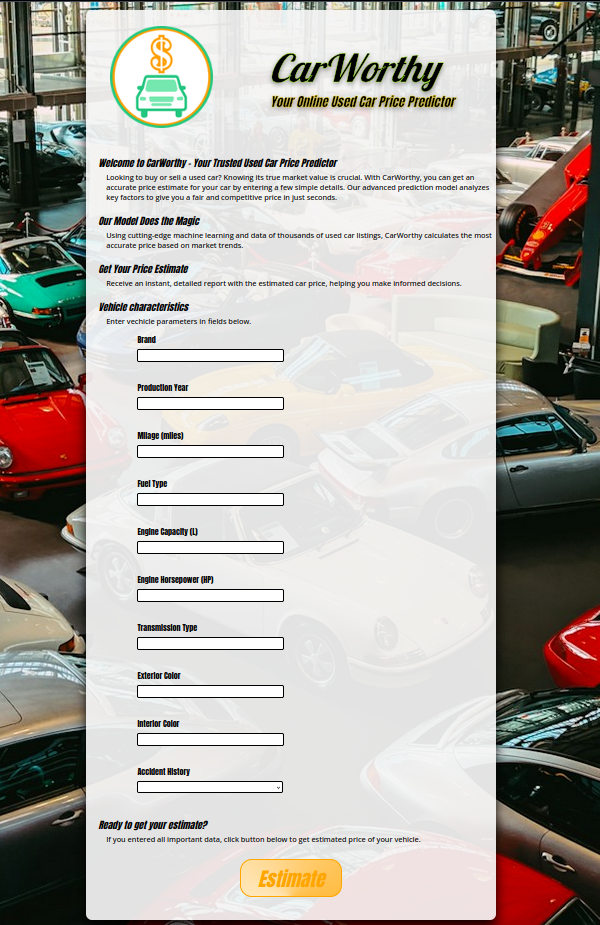
\includegraphics[width=0.9\textwidth]{images/page_view}
    \caption{Widok strony}
\end{figure}
\subsection{Okno z ceną}
\begin{figure}[H]
    \centering
    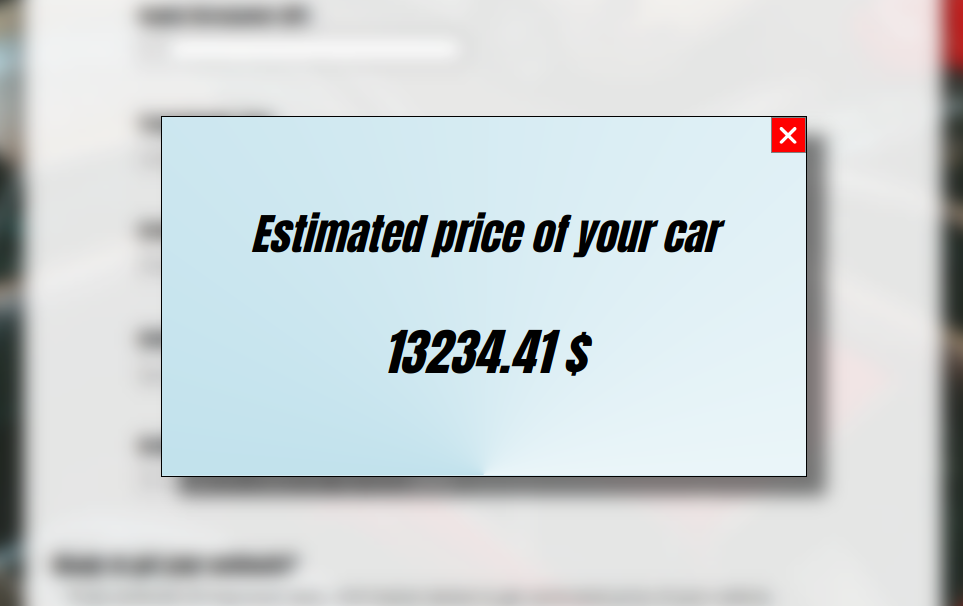
\includegraphics[width=0.9\textwidth]{images/price_view}
    \caption{Widok okna z ceną}
\end{figure}
\subsection{Okno z błędem}
\begin{figure}[H]
    \centering
    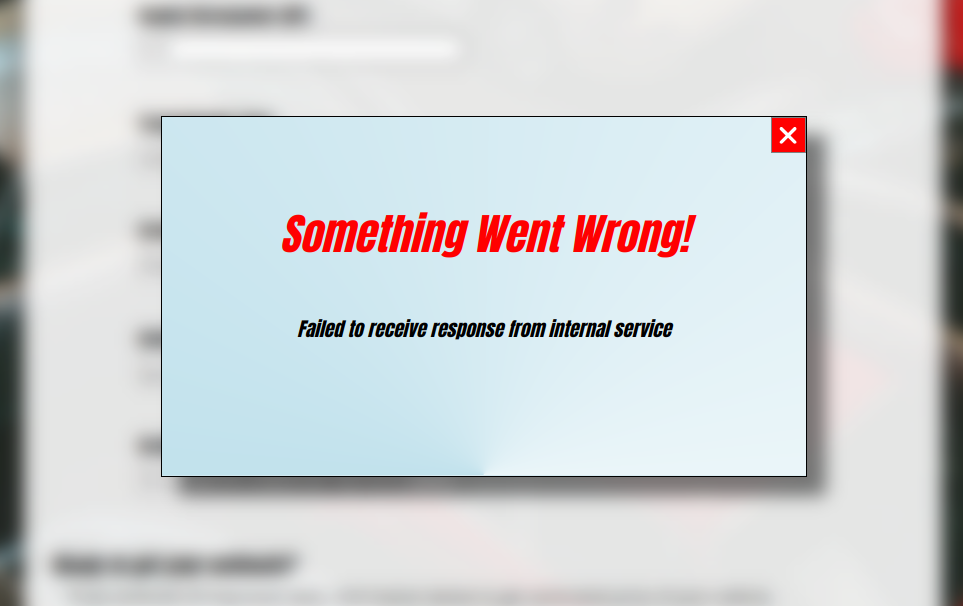
\includegraphics[width=0.9\textwidth]{images/error_view}
    \caption{Widok okna z błędem}
\end{figure}


\chapter{Komponent pośredniczący}
\section{Opis}
Komponent pośrediczący pełni rolę pośrednika pomiędzy aplikacją kliencką i serwisem predykcyjnym.
Otrzymywane od \textbf{frontendu}\footnote{Część aplikacji, z którą użytkownik wchodzi w bezpośednią interakcję, w tym wszystko co widzi oraz elementy wizualne i interaktywne.}
dane w formie \textbf{JSON}\footnote{JavaScript Object Notation --- format danych zapewniający kompaktowe rozmiary i jest czytelny dla ludzi i maszyn.}
są w tym komponencie przetwarzane na wiadomości w formacie odpowiadającym wejściu modelu, z uwzględnieniem procesu \textbf{kodowania liczbowego}\footnote{
Technika zamiany wartości danych tekstowych na wartości liczbowe, poprzez przypisanie unikalnej liczby każdej unikalnej wartości tekstowej.
} pól. Otrzymane w tym procesie wiadomości zapisywane są na \textbf{temat}\footnote{Podstawowy komponent Apache Kafka służący do kategoryzacji napływających wiadomości.}
 wejściowy Kafki. Pośrednik jest również odpowiedzialny za odczytywanie danych z tematu wyjściowego i
przekazywanie uzyskanych z nich informacji do klienta.
\section{Technologie}
\begin{itemize}
    \item Java --- Obiektowy język programowania.
    \item SpringBoot --- Framework dla języka Java nastawiony na wytwarzanie aplikacji webowych i mikroserwisów
    \item Gradle --- Narzędzie do automatyzacji budowania projektów.
\end{itemize}
\chapter{Komponent komunikacyjny}
\section{Opis}
Komponent komunikacyjny odpowiedzialny jest za transport danych pomiędzy komponentem pośredniczącym i serwisem predykcyjnym.
Wykorzystuje w tym celu skonteneryzowany \textbf{broker}\footnote{Serwer Apache Kafka zawierający dane należące do tematów i partycji, na które może być podzielony temat.}
wiadomości Apache Kafka wraz z dwoma tematami: input oraz output, wykorzystywanych
odpowiednio do gromadzenia danych odczytywanych przez serwis predykcyjny i gromadzenia danych odczytywanych przez pośrednika.
Do zarządzania brokerem wykorzystywany jest Apache Zookeeper.
\section{Technologie}
\begin{itemize}
    \item Apache Kafka --- Platforma przetwarzania danych w czasie rzeczywistym.
    \item Apache Zookeeper --- Usługa koordynacyjna systemów rozproszonych.
\end{itemize}

\chapter{Przygotowanie danych}
\section{Opis}
    Model jest skuteczny, gdy dane na których się go trenuje są odpowiednio przygotowane. Początkowo należy przeanalizować potencjalne zagrożenia w postaci braków poszczególnych wartości w polach danych oraz wartości odstających, mogących zniekształcić miary statystyczne. Na końcu należy zfaktoryzować, a zatem znumeryzować dane kategoryczne tak aby model mógł się na nich uczyć.

\section{Wizualizacja danych}
    \subsection*{Kilka wykresów pokazujących zbiór danych}
    \begin{figure}[H]
    \centering
    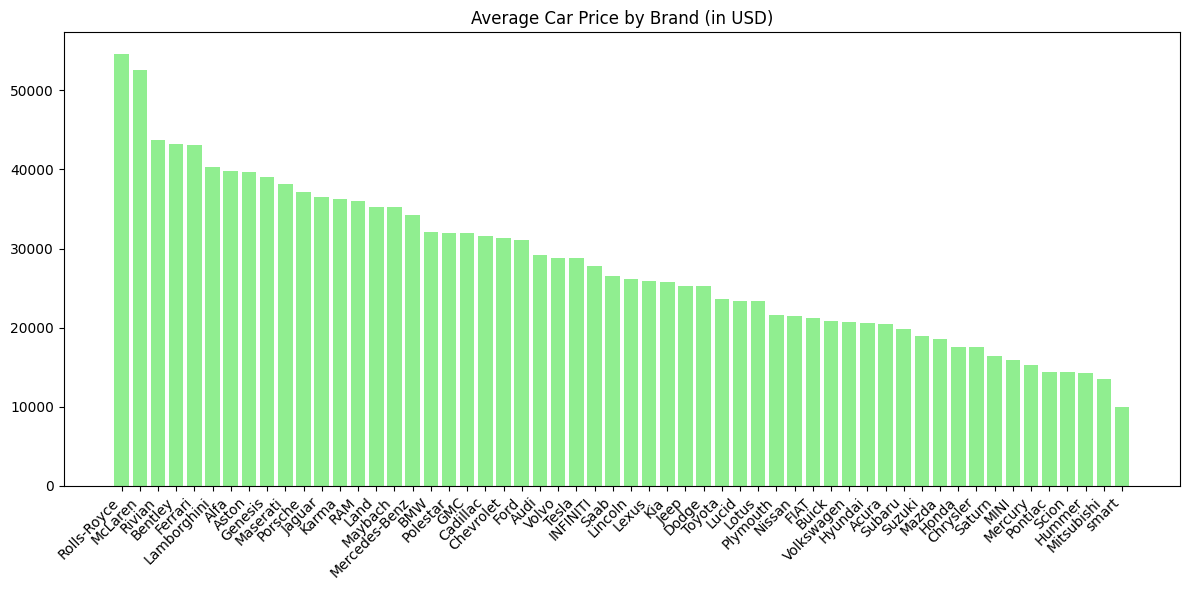
\includegraphics[width=0.9\textwidth]{images/avg_car_price_by_brand.png}
    \caption{Średnia cena pojazdu danej marki}
    \end{figure}
    \begin{figure}[H]
    \centering
    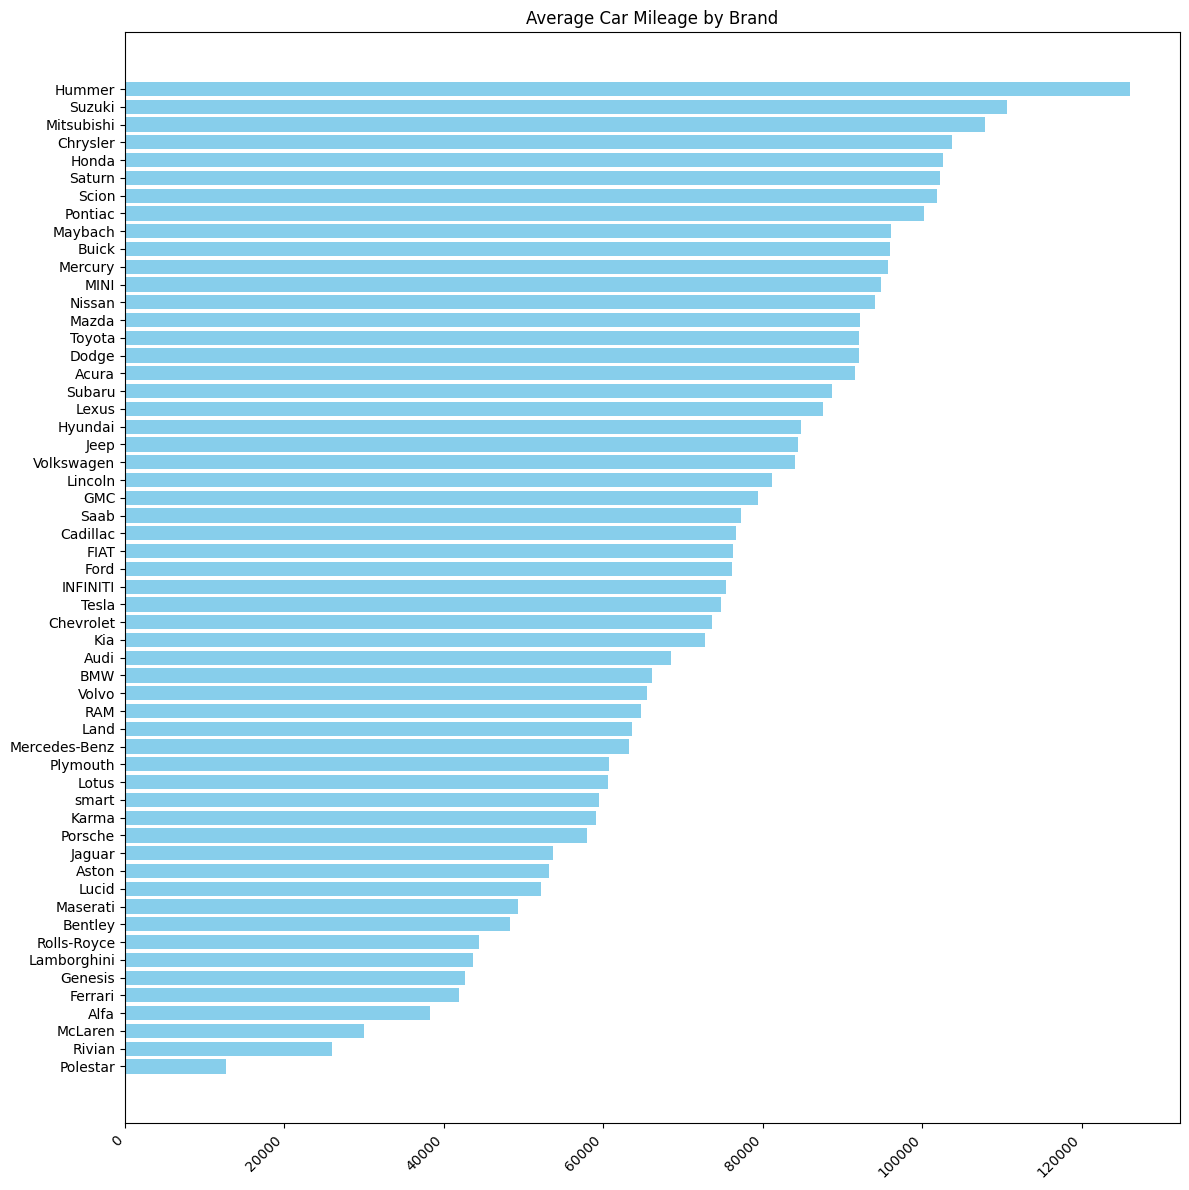
\includegraphics[width=0.9\textwidth]{images/avg_mileage_by_car_brand.png}
    \caption{Średnia ilość przejechanych mil pojazdów danej marki}
    \end{figure}
    \begin{figure}[H]
    \centering
    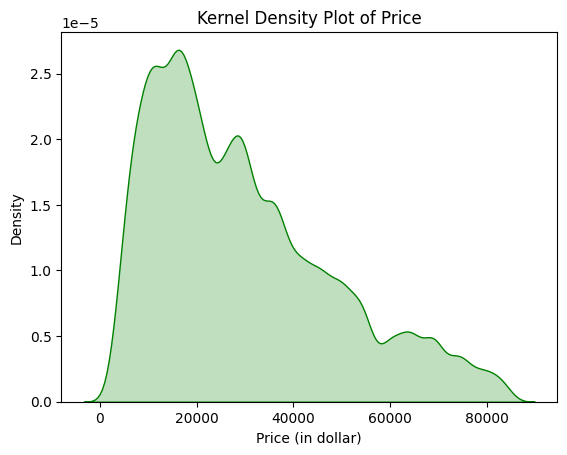
\includegraphics[width=0.9\textwidth]{images/density_price.png}
    \caption{Wykres gęstości cen pojazdów, widać że najwięcej jest ich w okolicach 17 tyś. USD}
    \end{figure}
\section{Puste pola}
    Postanowiliśmy usunąć puste pola zamiast stosować inne metody sztucznego ich wypełniania na przykład średnią, ponieważ zestaw danych jest obszerny i usunięcie próbek z pustymi wartościami nie odbije się na dokładności modelu.
\begin{table}[h!]
\centering
\begin{tabular}{|l|c|}
\hline
Przed usunięciem wartości odstających   & 188533 \\ \hline
Po usunięciu wartości odstających       & 162610 \\ \hline
\end{tabular}
\caption{Wielkość zbioru danych przed i po usunięciu wartości odstających}
\label{tab:wielkosc_zbioru}
\end{table}
    
\section{Zestaw danych z wartościami odstającymi}
\begin{figure}[H]
    \centering
    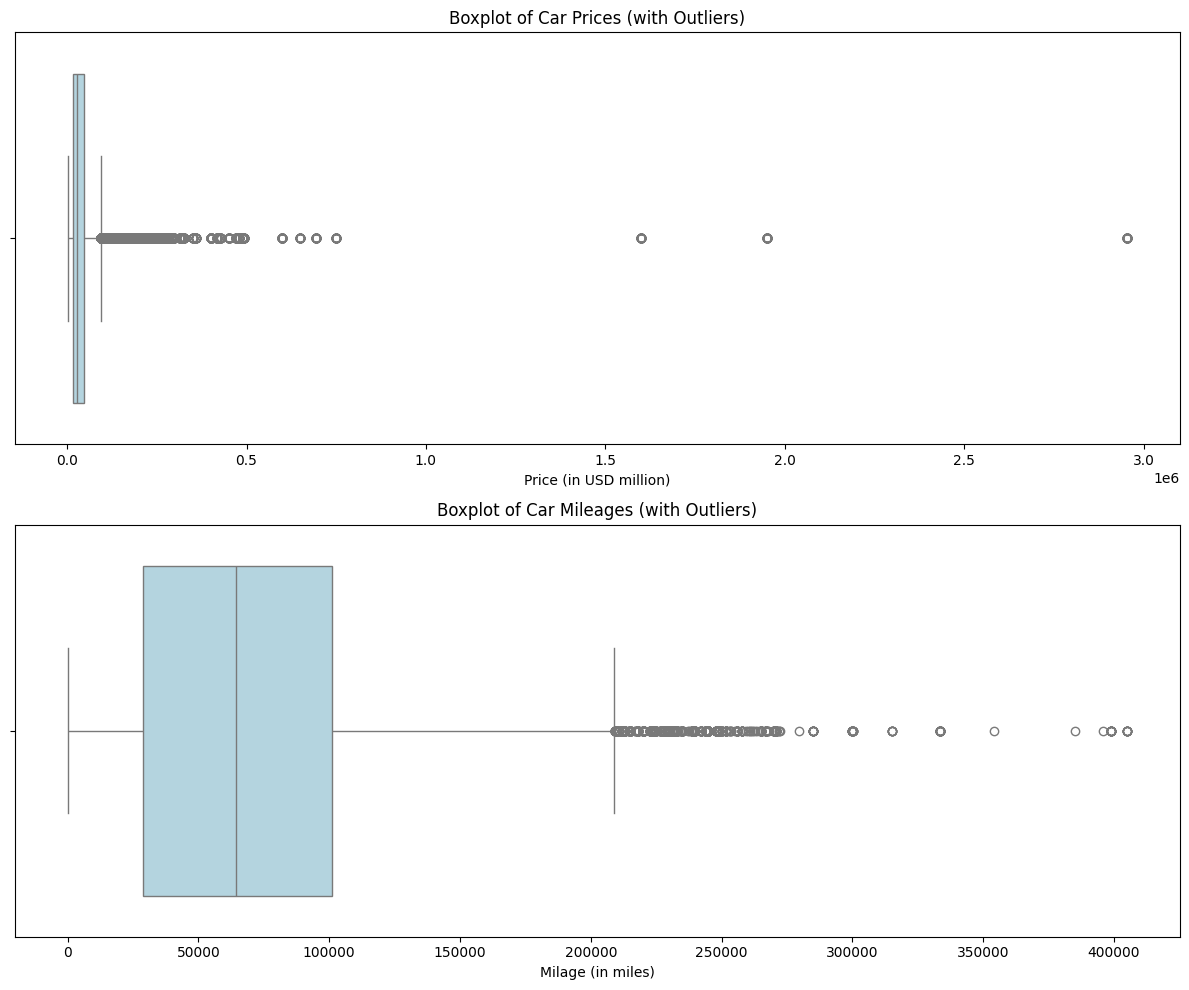
\includegraphics[width=0.9\textwidth]{images/boxplots_with_outlires.png}
    \caption{Niektóre wartości są zbyt duże, należy się ich pozbyć}
\end{figure}
\section{Wykrywanie i usuwanie wartości odstających za pomocą metody IQR}

Aby wykryć i usunąć wartości odstające w zbiorze danych na podstawie kolumn \texttt{price} oraz \texttt{milage}, wykonaliśmy następujące kroki:

\subsection*{1. Obliczenie kwartyli}
Pierwszy kwartyl ($Q_1$) oraz trzeci kwartyl ($Q_3$) wyznaczane są dla każdej kolumny. Odpowiadają one 25. i 75. percentylowi:
\[
Q_1 = \text{25. percentyl}, \quad Q_3 = \text{75. percentyl}
\]
\subsection*{2. Obliczenie rozstępu międzykwartylowego (IQR)}
Rozstęp międzykwartylowy (IQR) oblicza się jako:
\[
IQR = Q_3 - Q_1
\]
\subsection*{3. Definiowanie granic wartości odstających}
Wartości odstające to te, które znajdują się poza przedziałem:
\[
\text{Dolna granica} = Q_1 - 1.5 \cdot IQR, \quad \text{Górna granica} = Q_3 + 1.5 \cdot IQR
\]
Dla kolumn \texttt{price} oraz \texttt{milage} wyznacza się odpowiednio:
\[
\text{Dolna granica}_{\text{price}} = Q_{1,\text{price}} - 1.5 \cdot IQR_{\text{price}}, \quad \text{Górna granica}_{\text{price}} = Q_{3,\text{price}} + 1.5 \cdot IQR_{\text{price}}
\]
\[
\text{Dolna granica}_{\text{milage}} = Q_{1,\text{milage}} - 1.5 \cdot IQR_{\text{milage}}, \quad \text{Górna granica}_{\text{milage}} = Q_{3,\text{milage}} + 1.5 \cdot IQR_{\text{milage}}
\]
\subsection*{4. Filtrowanie wierszy bez wartości odstających}
Zbiór danych jest filtrowany w taki sposób, aby wartości w kolumnach \texttt{price} oraz \texttt{milage} spełniały następujące warunki:
\[
Q_1 - 1.5 \cdot IQR \leq X \leq Q_3 + 1.5 \cdot IQR
\]

\section{Zestaw danych bez wartości odstających}
\begin{figure}[H]
    \centering
    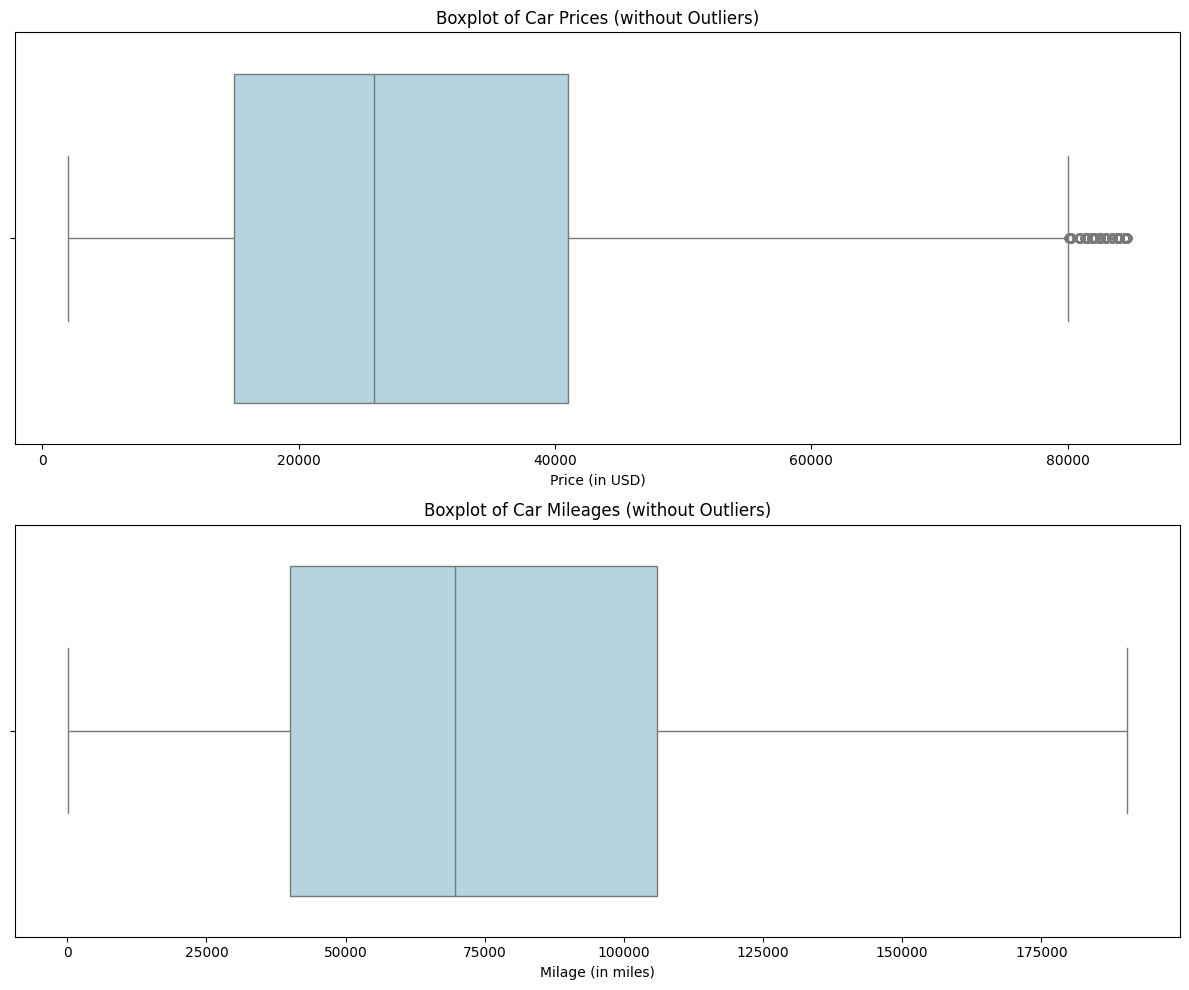
\includegraphics[width=0.9\textwidth]{images/boxplots_without_outlires.png}
    \caption{Brak lub mała ilość wartości odstających}
\end{figure}
\section{Wyodrębnienie znaczących informacji o silniku}

W zestawie danych istniała kolumna o nazwie \texttt{engine}, w której wartości przedstawiały krótki opis silnika, zawierający takie informacje jak liczba koni mechanicznych, pojemność silnika oraz inne cechy. Przykładowy opis to:

\begin{quote}
\texttt{172.0HP 1.6L 4 Cylinder Engine Gasoline Fuel}
\end{quote}

Z takiego opisu, za pomocą wyrażeń regularnych, wyodrębniliśmy dwie główne informacje: pojemność silnika oraz liczbę koni mechanicznych. 

Dla przykładu:
\[
\texttt{172.0HP 1.6L 4 Cylinder Engine Gasoline Fuel} \quad \rightarrow \quad 1.6, \ 172.0
\]

\subsection*{Zastąpienie kolumny \texttt{engine} nowymi kolumnami:}
Po wyodrębnieniu informacji o pojemności silnika oraz liczbie koni mechanicznych, zastąpiliśmy istniejącą kolumnę \texttt{engine} dwiema nowymi kolumnami:
\begin{itemize}
    \item \texttt{engine\_horsepower} – zawierającą moc silnika w koniach mechanicznych (HP).
    \item \texttt{engine\_capacity} – zawierającą pojemność silnika w litrach (L).
\end{itemize}

\section{Faktoryzacja danych}
    Modele uczenia maszynowego wymagają danych numerycznych jako wejścia. Wartości tekstowe (kategoryczne) muszą być przekonwertowane na liczby w sposób, który zachowa sens danych, ale jednocześnie nie wprowadzi sztucznej relacji między kategoriami. Do każdej wartości kategorycznej został przypisany numer, następnie dzięki słownikowi zamieniliśmy wszystkie próbki w wektory cech w następujący sposób:

\subsection*{Dane przed faktoryzacją}
Przykład danych wejściowych przed faktoryzacją:

\begin{lstlisting}[language=json, frame=single, basicstyle=\ttfamily\small, backgroundcolor=\color{lightgray}, stepnumber=1, numbersep=5pt]
{
  "brand": "Toyota",
  "transmission": "Automatic",
  "fuel_type": "Gasoline",
  "ext_col": "Red",
  "int_col": "White",
  "accident": "No accident",
}
\end{lstlisting}

\subsection*{Dane po faktoryzacji}
Po zastosowaniu faktoryzacji 'Label-Encoding' (przypisaniu liczb do kategorii), dane będą wyglądać następująco:

\begin{lstlisting}[language=json, frame=single, basicstyle=\ttfamily\small, backgroundcolor=\color{lightgray}, stepnumber=1, numbersep=5pt]
{
  "brand": 5,
  "transmission": 0,
  "fuel_type": 0,
  "ext_col": 3,
  "int_col": 5,
  "accident": 0,
}
\end{lstlisting}

\subsection*{Przykładowy wiersz danych po faktoryzacji:}

\begin{longtable}{|l|r|}
\hline
\textbf{Nazwa zmiennej} & \textbf{Wartość} \\
\hline
\endfirsthead
\hline
\textbf{Nazwa zmiennej} & \textbf{Wartość} \\
\hline
\endhead
\hline
\endfoot
\hline
\endlastfoot
model\_year & 2002 \\
milage & 143250.0 \\
price & 4999 \\
engine\_capacity & 3.9 \\
engine\_horsepower & 252.0 \\
brand\_numeric & 17.0 \\
transmission\_numeric & 0.0 \\
fuel\_type\_numeric & 0.0 \\
ext\_col\_numeric & 3.0 \\
int\_col\_numeric & 1.0 \\
accident\_numeric & 1.0 \\
\end{longtable}

\begin{figure}[H]
    \centering
    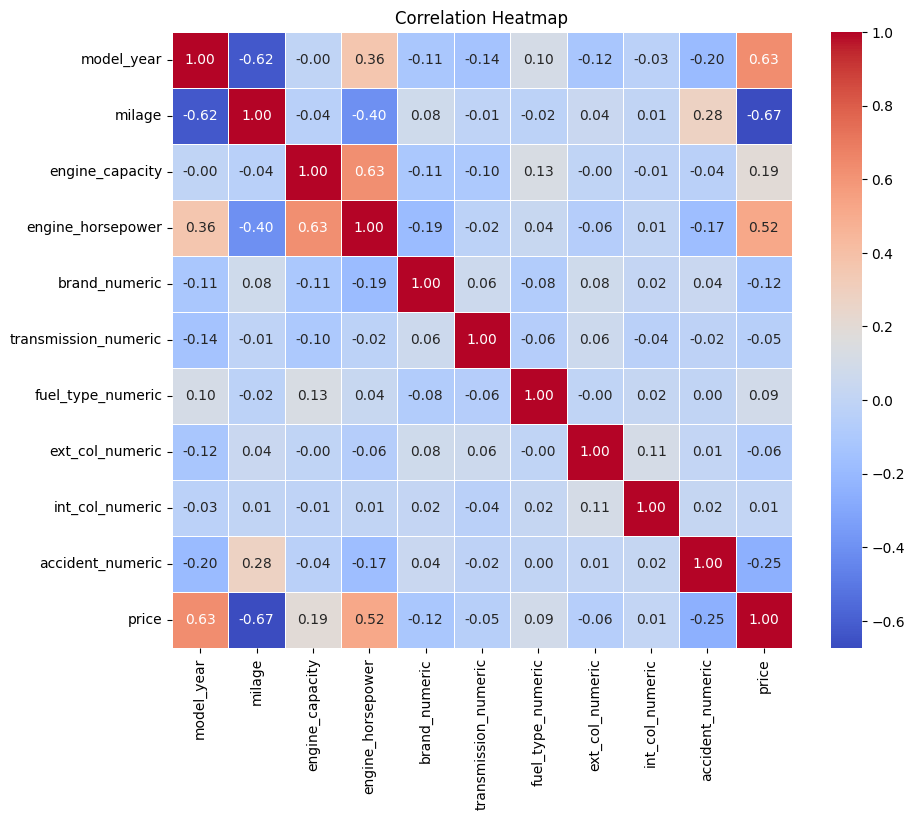
\includegraphics[width=0.9\textwidth]{images/correlation_heatmap.png}
    \caption{Macierz korelacji wszystkich cech, cechy korelującę się w największym stopniu z ceną: rok produkcji modelu, przebieg samochodu oraz konie mechaniczne}
\end{figure}

\chapter{Serwis predykcyjny}
\section{Opis}
    Zadaniem serwisu predykcyjnego jest dokonanie predykcji ceny samochodu na podstawie dostarczonego zestawu cech.
    W tym celu wykorzystuje gotowy, zapisany model przygotowany przy użyciu modułu SparkML.\@
    Dane przekazywane do modelu są odczytywane z tematu input za pomocą frameworka Spark. Cena zwrócona przez
    model zostaje zapisana na temat wyjściowy output.
\section{Technologie}
\begin{itemize}
    \item Python --- Język skryptowy. 
    \item Apache Spark --- Framework do sprawnego przetwarzania zbiorów danych w pamięci.
    \item Apache SparkML --- Moduł Apache Spark przeznaczony do uczenia maszynowego.
\end{itemize}

\section{Wybór modelu}

Podczas wyboru modelu kierowaliśmy się strukturą danych. Skorzystaliśmy z \textbf{Label Encoding}, czyli przypisania unikalnych wartości liczbowych dla każdej kategorii, np.:
\begin{quote}
\texttt{"BMW" $\rightarrow$ 0}, \texttt{"Audi" $\rightarrow$ 1}.
\end{quote}

\noindent W tym przypadku \textbf{modele regresji liniowej} nie są skuteczne, ponieważ takie kodowanie może prowadzić do błędnych założeń o istnieniu relacji liczbowych między kategoriami. Przykładowo:
\[
\text{Różnica między 0 a 1} = \text{Różnica między 1 a 2},
\]
co nie ma sensu w przypadku zmiennych kategorycznych.

\noindent \textbf{Rozwiązaniem są modele oparte na drzewach decyzyjnych}, takie jak:
\begin{itemize}
    \item Drzewo decyzyjne,
    \item Las losowy.
\end{itemize}

\section{Testowanie modeli}

\subsection{Las Losowy}

\noindent Do testowania modeli użyliśmy metod z biblioteki \texttt{pyspark.ml.tuning}.  
Jednym z kluczowych kroków było zdefiniowanie siatki hiperparametrów za pomocą \textbf{ParamGridBuilder}.

\vspace{0.5em}

\noindent \textbf{Definiowanie siatki hiperparametrów:}
\begin{lstlisting}[caption={Siatka hiperparametrów dla modelu}]
paramGrid = ParamGridBuilder() \
    .addGrid(rf.numTrees, [50, 100]) \
    .addGrid(rf.maxDepth, [5, 10]) \
    .addGrid(rf.minInstancesPerNode, [1, 2, 4]) \
    .addGrid(rf.maxBins, [32, 64, 128]) \
    .addGrid(rf.subsamplingRate, [0.5, 0.7, 1.0]) \
    .addGrid(rf.featureSubsetStrategy, ['all', 'sqrt', 'log2']) \
    .build()
\end{lstlisting}

\vspace{1em}

\noindent \textbf{Tworzenie obiektu ewaluatora:}  
Aby obliczyć dokładność modelu według metryki RMSE (Root Mean Squared Error), użyliśmy \texttt{RegressionEvaluator}.

\begin{lstlisting}[caption={Ewaluator dla metryki RMSE}]
evaluator_rmse = RegressionEvaluator(
    labelCol="price",
    predictionCol="prediction",
    metricName="rmse"
)
\end{lstlisting}

\vspace{1em}

\noindent \textbf{Walidacja krzyżowa:}  
W celu strojenia hiperparametrów wykorzystaliśmy \texttt{CrossValidator}, który przeprowadza walidację krzyżową z podziałem na \( K \)-podbiorów.  
Technika ta polega na:
\begin{enumerate}
    \item Podziale danych na \( K \)-podzbiorów (folds),
    \item Trenowaniu modelu \( K \)-razy na \( K-1 \)-podzbiorach,
    \item Użyciu pozostałego podzbioru do walidacji,
    \item Uśrednieniu wyników dla ostatecznej oceny modelu.
\end{enumerate}

\begin{lstlisting}[caption={CrossValidator do walidacji krzyżowej}]
crossval = CrossValidator(
    estimator=rf,
    estimatorParamMaps=paramGrid,
    evaluator=evaluator_rmse,
    numFolds=3  # 3-fold cross-validation
)
\end{lstlisting}

\vspace{1em}

\noindent \textbf{Uczenie modelu:}  
Najlepszy model z najmniejszym RMSE został zapisany do zmiennej \texttt{best\_model}.

\begin{lstlisting}[caption={Uczenie modelu i wybór najlepszego}]
cv_model = crossval.fit(train_data)
best_model = cv_model.bestModel
\end{lstlisting}

\subsection*{Najlepsze znalezione parametry Lasu losowego}
\noindent
\begin{center}
\begin{tabular}{l l}
\toprule
\textbf{Parametr}             & \textbf{Wartość} \\ 
\midrule
NumTrees                      & 100              \\
MaxDepth                      & 10               \\
MinInstancesPerNode           & 4                \\
MaxBins                       & 64               \\
SubsamplingRate               & 0.5              \\
FeatureSubsetStrategy         & sqrt             \\
MaxMemoryInMB                 & 256              \\
\bottomrule
\end{tabular}
\end{center}

\vspace{1em}

\noindent \textbf{Czas trenowania:}  
\large{116 minut}

\vspace{1em}

\subsection*{Metryki ewaluacyjne dla powyższych hiperparametrów}
\begin{center}
\begin{tabular}{l l}
\toprule
\textbf{Metryka}              & \textbf{Wartość} \\ 
\midrule
Root Mean Squared Error (RMSE) & 11011.20         \\
Mean Absolute Error (MAE)     & 7962.28          \\
R-squared (R\textsuperscript{2}) & 0.6625          \\
\bottomrule
\end{tabular}
\end{center}

\subsection{Drzewo decyzyjne}
\textbf{Definiowanie siatki hiperparametrów:}
\begin{lstlisting}[caption={Siatka hiperparametrów dla modelu drzewa decyzujnego}]
paramGrid = ParamGridBuilder() \
    .addGrid(dt.maxDepth, [10, 15]) \
    .addGrid(dt.maxBins, [20, 30, 40]) \
    .addGrid(dt.minInstancesPerNode, [1, 2, 4]) \
    .addGrid(dt.minInfoGain, [0.0, 0.1, 0.2]) \
    .addGrid(dt.maxMemoryInMB, [512, 1024]) \
    .addGrid(dt.cacheNodeIds, [True, False]) \
    .addGrid(dt.checkpointInterval, [10, 20]) \
    .build()
\end{lstlisting}
\noindent \textbf{Obiekt ewaluatora oraz walidacji krzyżowej są takie same jak w przypdaku Lasu losowego}

\subsection*{Najlepsze znalezione parametry Drzewa decyzyjnego}
\noindent
\begin{center}
\begin{tabular}{l l}
\toprule
\textbf{Parametr}             & \textbf{Wartość} \\ 
\midrule
MaxDepth                      & 10               \\
MaxBins                       & 20               \\
MinInstancesPerNode           & 4                \\
MinInfoGain                   & 0.0              \\
MaxMemoryInMB                 & 512              \\
CacheNodeIds                  & True             \\
CheckpointInterval            & 10               \\
\bottomrule
\end{tabular}
\end{center}

\vspace{1em}

\subsection*{Metryki ewaluacyjne dla powyższych hiperparametrów}

\noindent
\begin{center}
\begin{tabular}{l l}
\toprule
\textbf{Metryka}              & \textbf{Wartość} \\ 
\midrule
Root Mean Squared Error (RMSE) & 11318.40         \\
Mean Absolute Error (MAE)     & 8143.66          \\
R-squared (R\textsuperscript{2}) & 0.6434          \\
\bottomrule
\end{tabular}
\end{center}

\vspace{1em}

\noindent \textbf{Czas trenowania:}  
\large{66 minut}

\subsection{Podsumowanie}
    Na podstawie miar ewaluacji obu modeli, Las Losowy ma niewielką przewagę nad Drzewem decyzyjnym, jednak trening tego modelu oraz znalezienie najlepszych parametrów zająło blisko godzinę więcej.
\end{document}
